% =====================================================================
%  IIT Tirupati -- M.Tech Project (MTP) Poster Template
%  Project: Neural_Acc -- Activation-Sparse CNN Accelerator
%  Size: A1 portrait (594 mm x 841 mm)
%  Sections follow the evaluation points:
%    1 The challenge   2 Input   3 Output   4 Toughest problems solved
%    5 Critical challenges   6 Positioning vs existing work   7 Learnings
%  Compile: pdflatex poster_A1_portrait.tex  (Overleaf: pdfLaTeX)
%  Files needed in the same folder: this .tex file, iittp_logo.png,
%                                  Neural_Acc_Architecture_Presentation.png,
%                                  poster_results_chart.png
% =====================================================================
\documentclass{article}

% ---------- Page size: A1 portrait ----------
\usepackage[paperwidth=594mm,paperheight=841mm,margin=16mm]{geometry}

% ---------- Fonts ----------
\usepackage[T1]{fontenc}
\usepackage[scaled]{helvet}
\renewcommand{\familydefault}{\sfdefault}
\usepackage{sansmath}\sansmath

% ---------- Packages ----------
\usepackage{graphicx}
\usepackage{xcolor}
\usepackage[most]{tcolorbox}
\usepackage{booktabs}
\usepackage{enumitem}
\usepackage{amsmath}
\usepackage{pifont}
\usepackage{tikz}
\usetikzlibrary{arrows.meta,positioning}
\usepackage[hidelinks]{hyperref}
\pagestyle{empty}
\setlength{\parindent}{0pt}
\setlength{\parskip}{0.4em}

% ---------- IIT Tirupati colours (from the logo) ----------
\definecolor{iitmaroon}{HTML}{800000}
\definecolor{iitdark}{HTML}{1A1A1A}
\definecolor{iitlight}{HTML}{F7F2F2}
\definecolor{iitgray}{HTML}{5A5A5A}
\definecolor{iitgreen}{HTML}{1E7B34}
\color{iitdark}

% ---------- Font sizes for A1 (readable from ~1.5 m) ----------
\newcommand{\bodysize}{\fontsize{20}{27}\selectfont}
\newcommand{\headsize}{\fontsize{30}{36}\selectfont}
\newcommand{\titlesize}{\fontsize{52}{64}\selectfont}
\newcommand{\authorsize}{\fontsize{27}{35}\selectfont}
\newcommand{\affilsize}{\fontsize{21}{28}\selectfont}
\newcommand{\smallsize}{\fontsize{16}{21}\selectfont}
\newcommand{\bigsize}{\fontsize{26}{34}\selectfont}

% ---------- Lists ----------
\setlist[itemize]{leftmargin=1.2em, itemsep=0.2em, topsep=0.2em,
  label={\color{iitmaroon}\rule[0.2em]{0.42em}{0.42em}}}
\setlist[enumerate]{leftmargin=1.4em, itemsep=0.2em, topsep=0.2em,
  label={\color{iitmaroon}\bfseries\arabic*.}}

% ---------- Section box with a numbered badge ----------
\newcommand{\badge}[1]{%
  \ifx\relax#1\relax\else
  \tikz[baseline=(b.base)]\node[circle, fill=white, text=iitmaroon,
    inner sep=0pt, minimum size=1.15em, font=\bfseries](b){#1};\hspace{0.45em}\fi}

\newtcolorbox{posterblock}[3][]{%
  enhanced, colback=white, colframe=iitmaroon,
  boxrule=1.8pt, arc=4pt,
  left=14pt, right=14pt, top=10pt, bottom=12pt,
  toptitle=8pt, bottomtitle=8pt, lefttitle=14pt,
  coltitle=white, colbacktitle=iitmaroon,
  fonttitle=\headsize\bfseries,
  title={\badge{#2}#3},
  before skip=0pt, after skip=14pt,
  fontupper=\bodysize, #1}

% Highlighted statement box (left maroon bar)
\newtcolorbox{keybox}{%
  enhanced, colback=iitlight, colframe=iitmaroon,
  boxrule=0pt, leftrule=7pt, arc=0pt,
  left=14pt, right=12pt, top=8pt, bottom=8pt,
  fontupper=\bodysize\bfseries}

% Sub-heading inside a block
\newcommand{\subhead}[1]{{\color{iitmaroon}\bfseries #1}}
\newcommand{\figcaption}[1]{{\smallsize\color{iitgray}\textbf{Figure:} #1\par}}

% Tick and cross for the comparison table
\newcommand{\yes}{{\color{iitgreen}\ding{51}}}
\newcommand{\no}{{\color{iitmaroon}\ding{55}}}
\newcommand{\partly}{{\color{iitgray}$\sim$}}

% =====================================================================
\begin{document}

% ======================== HEADER ========================
\begin{minipage}[c]{0.18\textwidth}
  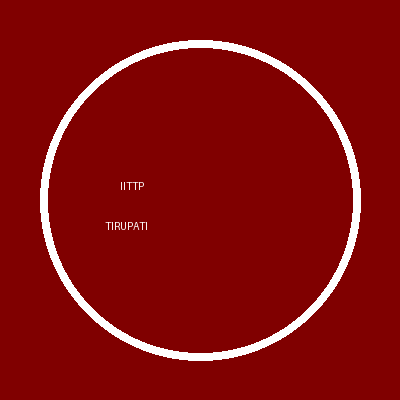
\includegraphics[width=\linewidth]{iittp_logo.png}
\end{minipage}%
\hfill
\begin{minipage}[c]{0.66\textwidth}
  \centering
  {\titlesize\bfseries\color{iitmaroon} SparseFlex: Activation-Sparse CNN Accelerator\\[0.1em]
   \fontsize{34}{42}\selectfont Reconfigurable 16/32/64-PE Array with Synchronous Zero-Gating \& Hardware Policy Interlocks\par}
  \vspace{0.4em}
  {\authorsize\bfseries Raushan Kumar (Roll No: CS23MXXX)\par}
  \vspace{0.2em}
  {\affilsize Supervisor: \textbf{Prof. Supervisor Name}\par}
  {\affilsize Department of Computer Science and Engineering, Indian Institute of Technology Tirupati\par}
  \vspace{0.1em}
  {\smallsize\color{iitgray} cs23mxxx@iittp.ac.in \quad | \quad Department of CSE, IIT Tirupati\par}
\end{minipage}%
\hfill
\begin{minipage}[c]{0.14\textwidth}
  \centering\begin{minipage}{0.9\linewidth}
  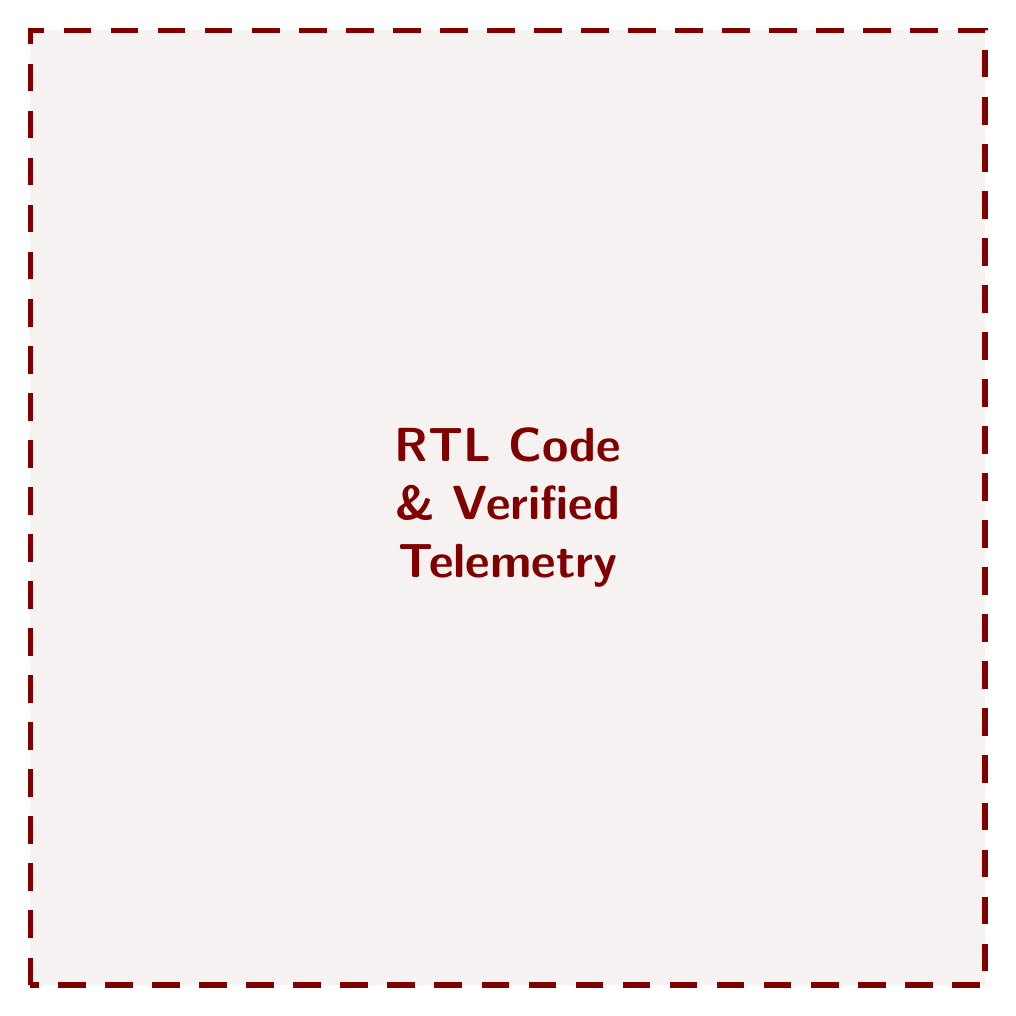
\begin{tikzpicture}
    \draw[iitmaroon, line width=2pt, dash pattern=on 10pt off 7pt, fill=iitlight]
      (0,0) rectangle (\linewidth,\linewidth);
    \node[text=iitmaroon, align=center, font=\smallsize\bfseries] at (0.5\linewidth,0.5\linewidth)
      {RTL Code\\ \& Verified\\ Telemetry};
  \end{tikzpicture}\end{minipage}
\end{minipage}

\vspace{10pt}
{\color{iitmaroon}\rule{\textwidth}{4.5pt}}
\vspace{12pt}

% ======================== 1. THE CHALLENGE ========================
\begin{posterblock}{1}{The Challenge}
{\bigsize\bfseries How can battery-powered edge systems execute deep CNN inference under real-time deadlines and dynamic thermal caps without wasting dynamic energy on ineffectual zero arithmetic?\par}
\vspace{0.25em}
\subhead{Why it matters:} Convolutional Neural Networks (CNNs) exhibit 40\%--85\% activation sparsity post-ReLU. Conventional sparse accelerators rely on \textbf{asynchronous zero-skipping}, causing severe spatial load imbalance, FIFO buffer congestion, and non-deterministic execution jitter. This unpredictability prevents deployment in safety-critical, hard real-time edge environments (autonomous robotics, automotive vision, UAVs).
\end{posterblock}

% ======================== 2 + 3. INPUT -> SYSTEM -> OUTPUT ========================
\begin{posterblock}{}{At a Glance: \;\badge{2}Input \;$\rightarrow$\; Our System \;$\rightarrow$\; \badge{3}Output}
\centering
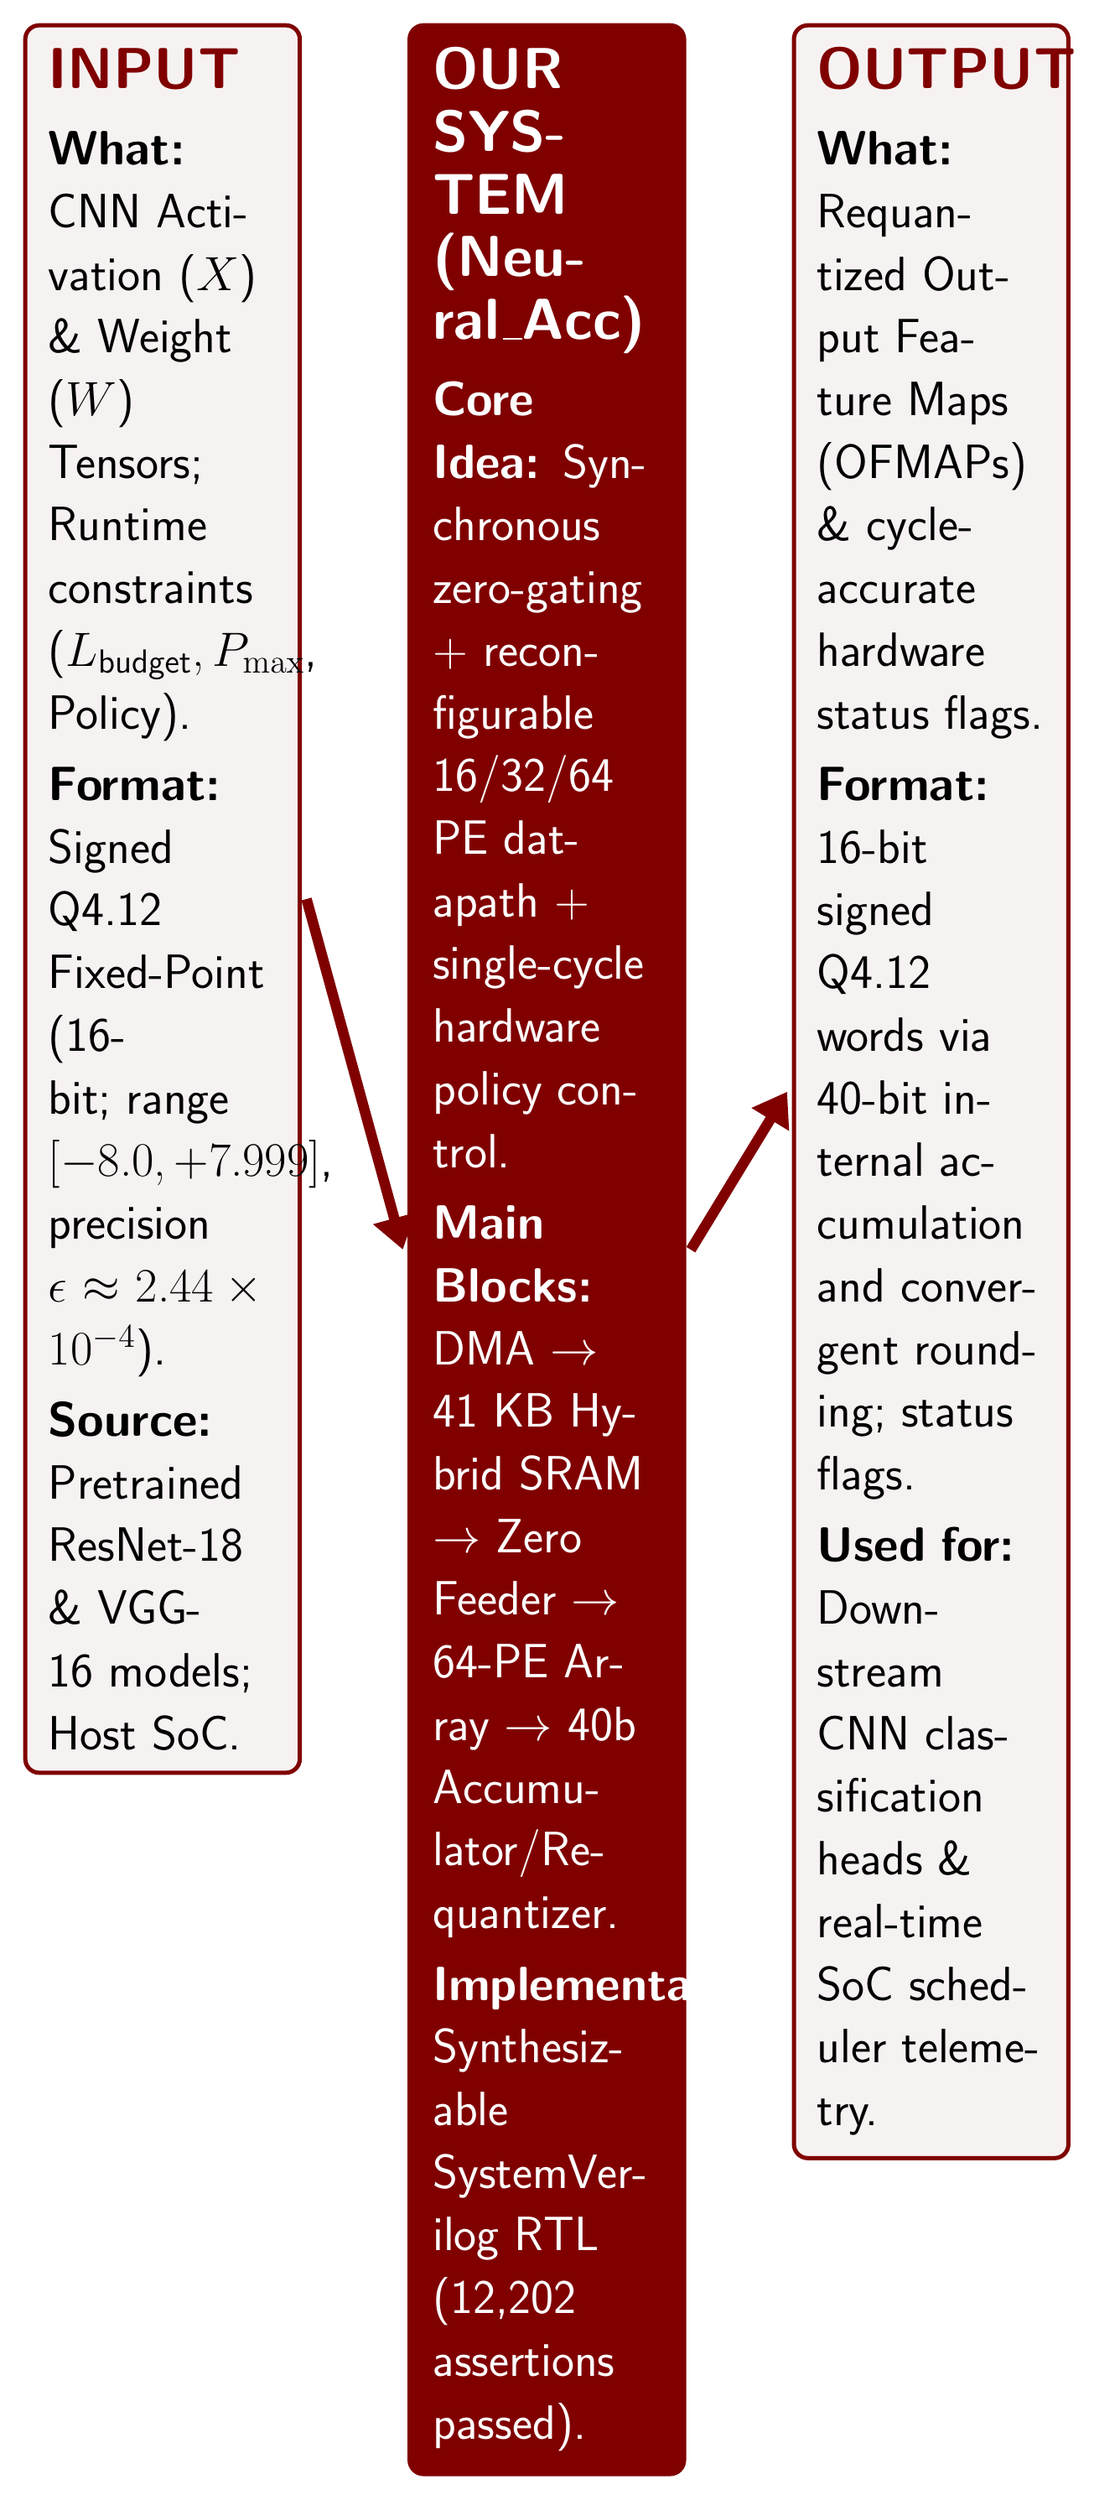
\begin{tikzpicture}[
    box/.style={draw=iitmaroon, line width=1.8pt, rounded corners=6pt,
      align=left, inner sep=10pt, minimum height=5.4cm, anchor=north west,
      font=\bodysize},
    arrow/.style={-{Triangle[length=14pt,width=18pt]}, line width=4.5pt, iitmaroon}]
  \node[box, fill=iitlight, text width=0.285\linewidth] (in) at (0,0)
    {{\headsize\bfseries\color{iitmaroon} INPUT}\\[0.3em]
     \textbf{What:} CNN Activation ($X$) \& Weight ($W$) Tensors; Runtime constraints ($L_{\text{budget}}, P_{\max}$, Policy).\\[0.2em]
     \textbf{Format:} Signed Q4.12 Fixed-Point (16-bit; range $[-8.0, +7.999]$, precision $\epsilon \approx 2.44 \times 10^{-4}$).\\[0.2em]
     \textbf{Source:} Pretrained ResNet-18 \& VGG-16 models; Host SoC.};
  \node[box, fill=iitmaroon, text=white, text width=0.285\linewidth,
        right=1.6cm of in.north east, anchor=north west] (sys)
    {{\headsize\bfseries OUR SYSTEM (Neural\_Acc)}\\[0.3em]
     \textbf{Core Idea:} Synchronous zero-gating + reconfigurable 16/32/64 PE datapath + single-cycle hardware policy control.\\[0.2em]
     \textbf{Main Blocks:} DMA $\rightarrow$ 41 KB Hybrid SRAM $\rightarrow$ Zero Feeder $\rightarrow$ 64-PE Array $\rightarrow$ 40b Accumulator/Requantizer.\\[0.2em]
     \textbf{Implementation:} Synthesizable SystemVerilog RTL (12,202 assertions passed).};
  \node[box, fill=iitlight, text width=0.285\linewidth,
        right=1.6cm of sys.north east, anchor=north west] (out)
    {{\headsize\bfseries\color{iitmaroon} OUTPUT}\\[0.3em]
     \textbf{What:} Requantized Output Feature Maps (OFMAPs) \& cycle-accurate hardware status flags.\\[0.2em]
     \textbf{Format:} 16-bit signed Q4.12 words via 40-bit internal accumulation and convergent rounding; status flags.\\[0.2em]
     \textbf{Used for:} Downstream CNN classification heads \& real-time SoC scheduler telemetry.};
  \draw[arrow] ([xshift=2pt]in.east) -- ([xshift=-2pt]sys.west);
  \draw[arrow] ([xshift=2pt]sys.east) -- ([xshift=-2pt]out.west);
\end{tikzpicture}
\end{posterblock}

% ======================== METHODOLOGY ========================
\begin{posterblock}{}{Proposed Methodology / System Architecture}
\begin{minipage}[t]{0.58\linewidth}\vspace{0pt}
\centering
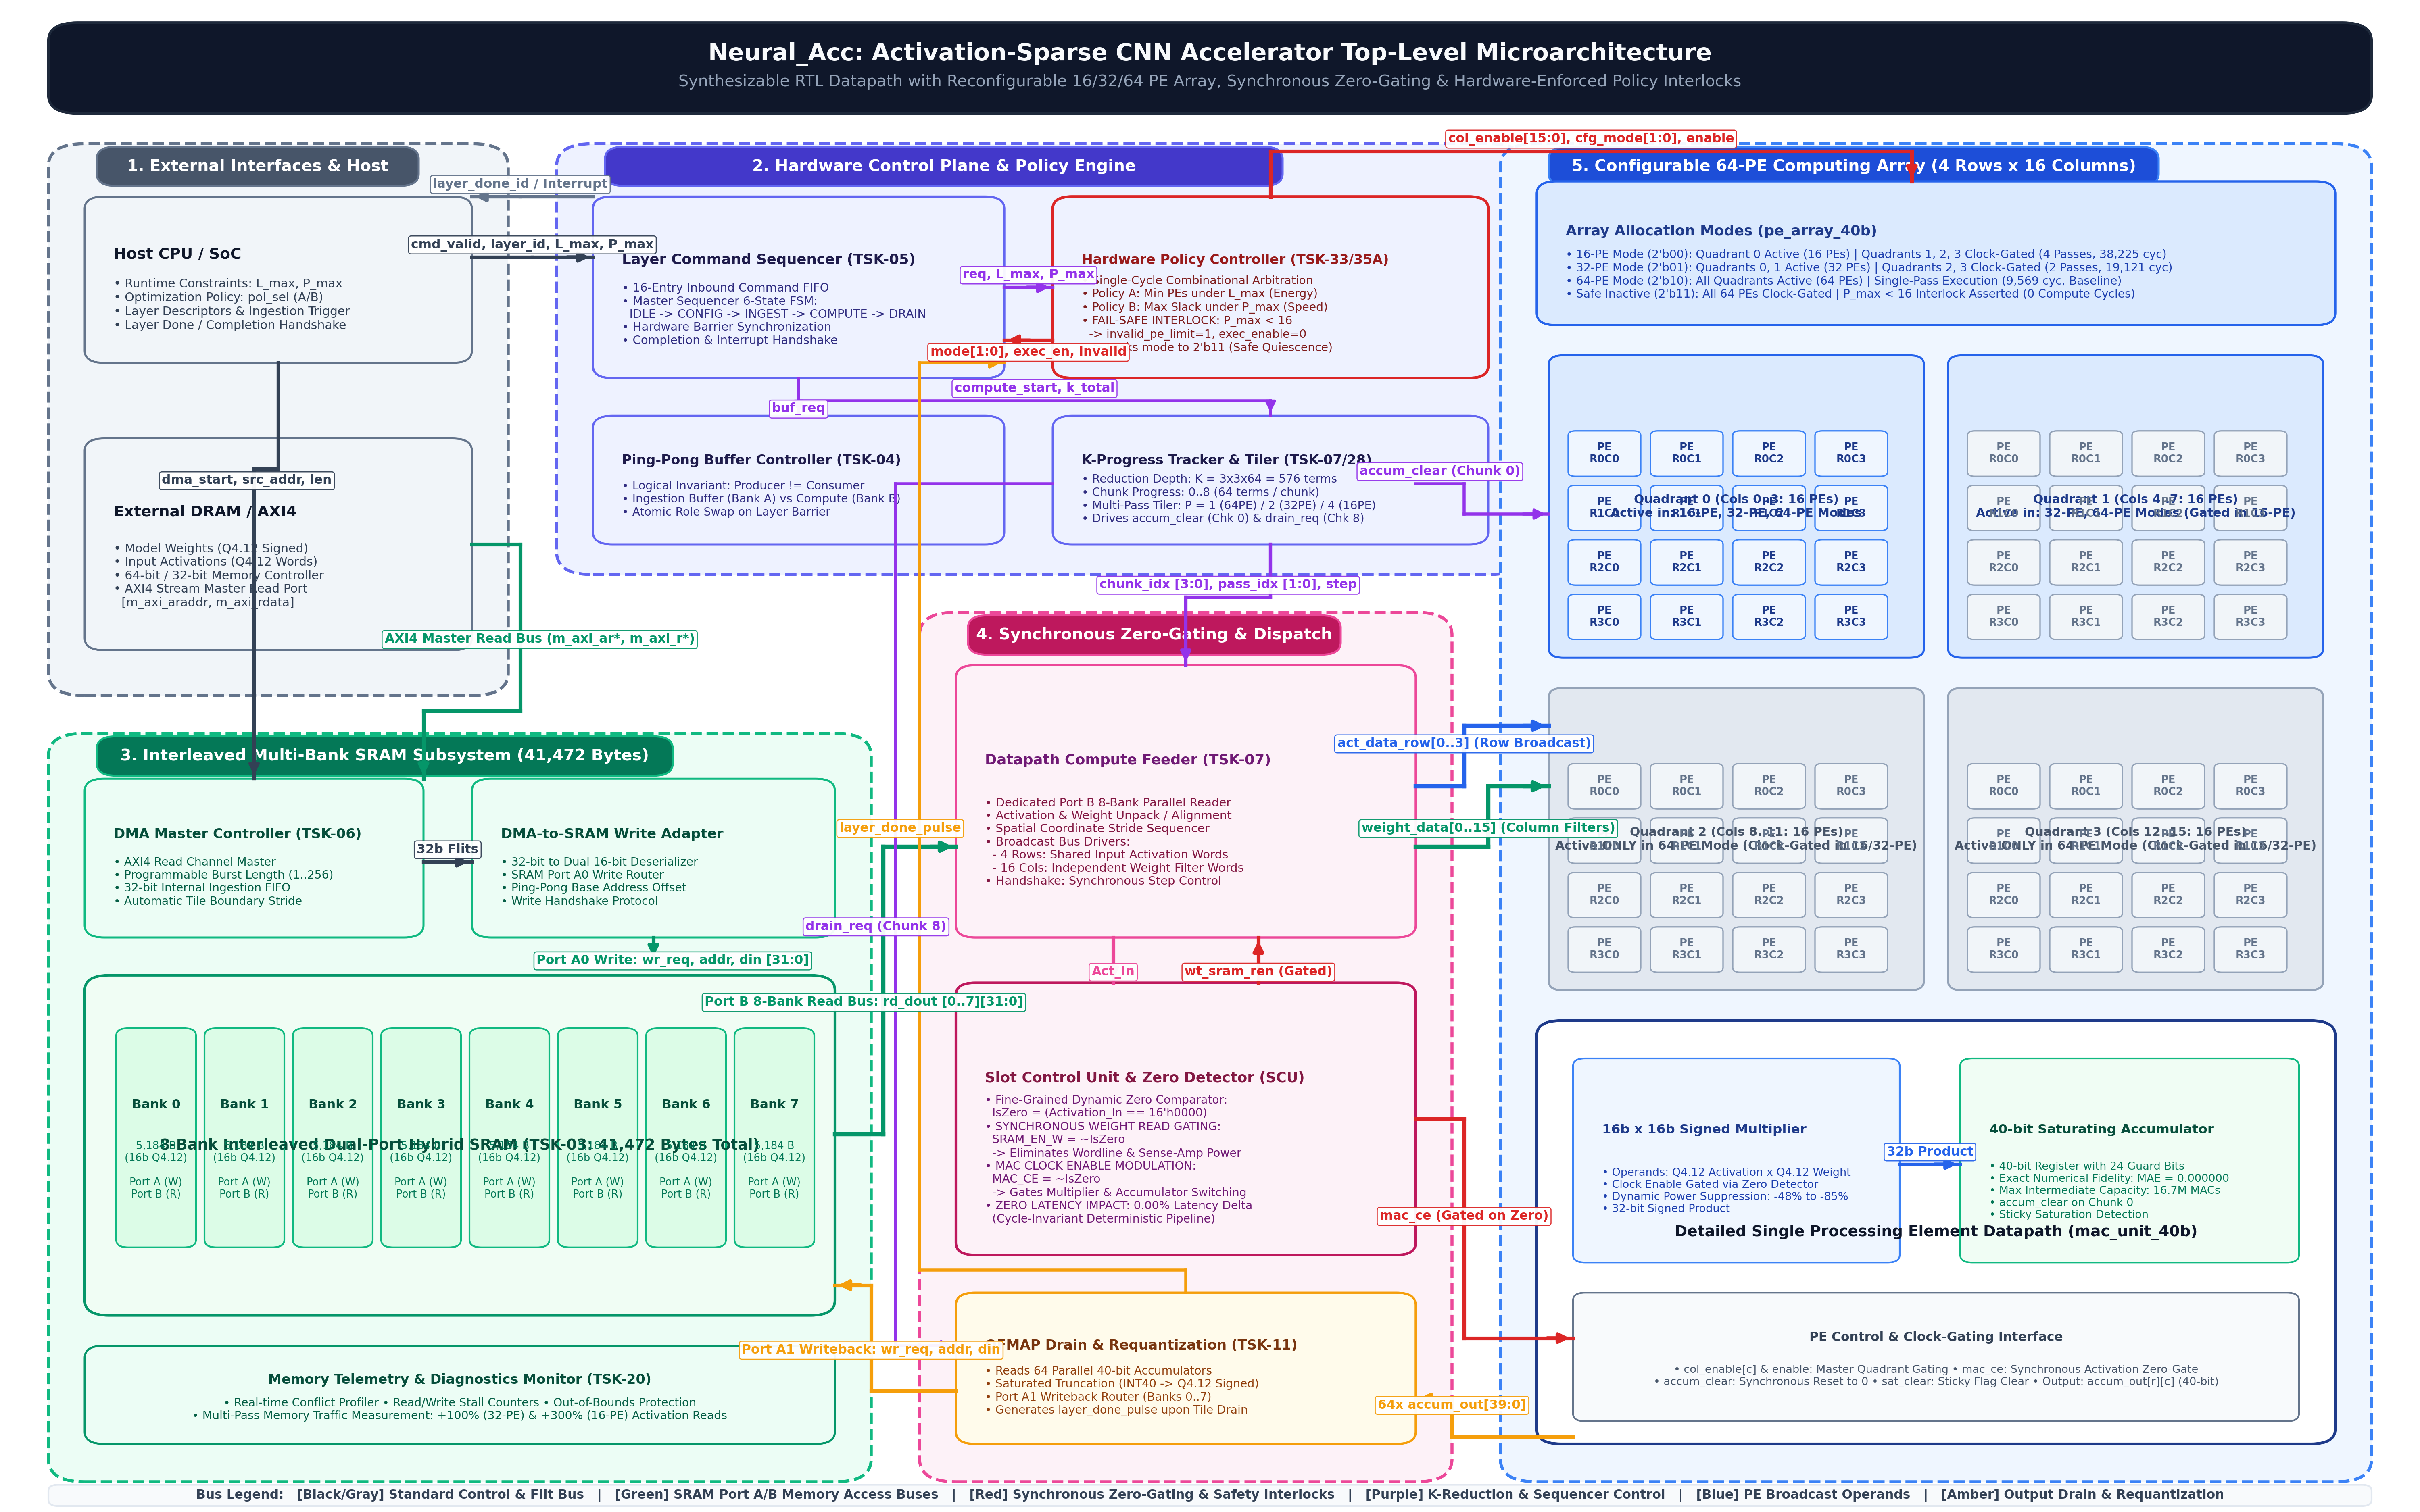
\includegraphics[width=\linewidth]{Neural_Acc_Architecture_Presentation.png}
\vspace{0.2em}
\figcaption{Neural\_Acc top-level microarchitecture showing 5 synchronized hardware subsystems.}
\end{minipage}%
\hfill
\begin{minipage}[t]{0.39\linewidth}\vspace{0pt}
\subhead{How it works in 3 Stages:}
\begin{enumerate}
  \item \textbf{Single-Cycle Policy Arbitration:} Combinatorial engine arbitrates between Policy A (min PEs under deadline) and Policy B (max slack); triggers hard fail-safe interlock if $P_{\max} < 16$.
  \item \textbf{Synchronous Zero-Gating:} Detects $A_{\text{in}} == 16\text{'h}0000$, suppressing weight SRAM read strobes and freezing PE multiplier clocks without altering pipeline timing.
  \item \textbf{Reconfigurable Tiling \& Drain:} Progressively clock-gates PE quadrants (saving 50\% or 75\% active logic) across $P = 64/N_{\text{active}}$ passes, accumulating in 40-bit registers before requantization.
\end{enumerate}
\vspace{0.3em}
\subhead{Governing Architectural Formulations:}
\[ \text{Active Logic Saved (\%)} = \left(\frac{64 - N_{\text{active}}}{64}\right) \times 100\%, \quad R_{\text{act}} = 9,216 \times \left(\frac{64}{N_{\text{active}}}\right) \]
{\smallsize $N_{\text{active}} \in \{16, 32, 64\}$: active PEs, $R_{\text{act}}$: activation SRAM reads, $P$: passes.\par}
\vspace{0.2em}
\subhead{Experimental Setup:} Evaluated across 4 real CNN layers (ResNet-18, VGG-16) on CIFAR-10/100; cycle-accurate SystemVerilog simulation against 64-bit golden model; AMD Vivado 2026.1 FPGA flow.
\end{minipage}
\end{posterblock}

% ======================== 4 + 5 ========================
\begin{minipage}[t]{0.488\textwidth}\vspace{0pt}
\begin{posterblock}[equal height group=rowA]{4}{Toughest Problems We Solved}
\subhead{P1. Strict Timing Determinism under Activation Sparsity}\\
\textbf{Problem:} Dynamic zero-skipping in literature destroys cycle predictability, causing queue congestion and severe spatial load imbalance.\\
\textbf{Solution:} Engineered a fully synchronous zero-detection engine that eliminates memory and arithmetic switching while pipeline counters advance uniformly.\\
\textbf{Gain:} \textbf{48.11\% to 84.92\%} reduction in weight reads and MAC switching with \textbf{0.00\% latency jitter} (strictly invariant 9,569 cycles).

\vspace{0.35em}
\subhead{P2. Discovering the Multi-Pass Memory Overhead}\\
\textbf{Problem:} Prior works claim PE downscaling delivers linear energy savings, ignoring on-chip memory access amplification.\\
\textbf{Solution:} Modeled and measured multi-pass channel tiling ($P = 64/N_{\text{active}}$) across dual-bank ping-pong SRAM.\\
\textbf{Gain:} Proved 16-PE scaling saves 75.0\% active logic but inflates activation SRAM reads by \textbf{+300\%} (36,864 vs. 9,216 reads), refuting naive energy proportionality claims.
\end{posterblock}
\end{minipage}%
\hfill
\begin{minipage}[t]{0.488\textwidth}\vspace{0pt}
\begin{posterblock}[equal height group=rowA]{5}{Critical Challenges Faced}
\begin{itemize}
  \item \textbf{Accumulator Dynamic Overflow ($K=576$):}\\
        $\rightarrow$ Sized 40-bit accumulators with 8 guard bits above product ($2^8 = 256$ full additions headroom), mathematically guaranteeing zero overflow (\textbf{MAE = 0.000000}).
  \item \textbf{Multi-Pass Sequencer FSM Race Conditions:}\\
        $\rightarrow$ Solved channel tiler and OFMAP drain handshake collisions by architecting an atomic 6-state Moore sequencer with barrier synchronization.
  \item \textbf{EDA Toolchain \& License Diagnostic Blocker:}\\
        $\rightarrow$ Pinpointed missing Vivado license via \texttt{xlicdiag.rpt}; created fully reproducible, automated Tcl power-estimation scripts.
  \item \textbf{Still open:} Standard-cell ASIC physical synthesis (e.g., TSMC 28nm) for sign-off silicon area and post-layout dynamic power.
\end{itemize}
\end{posterblock}
\end{minipage}

% ======================== RESULTS + 6 ========================
\begin{minipage}[t]{0.488\textwidth}\vspace{0pt}
\begin{posterblock}[equal height group=rowB]{}{Results and Analysis}
\begin{keybox}
Key result: SparseFlex successfully decouples power reduction from timing jitter, achieving up to \textbf{84.92\%} switching savings with \textbf{zero cycle variation} (0.00\% latency jitter).
\end{keybox}
\vspace{0.2em}
\centering
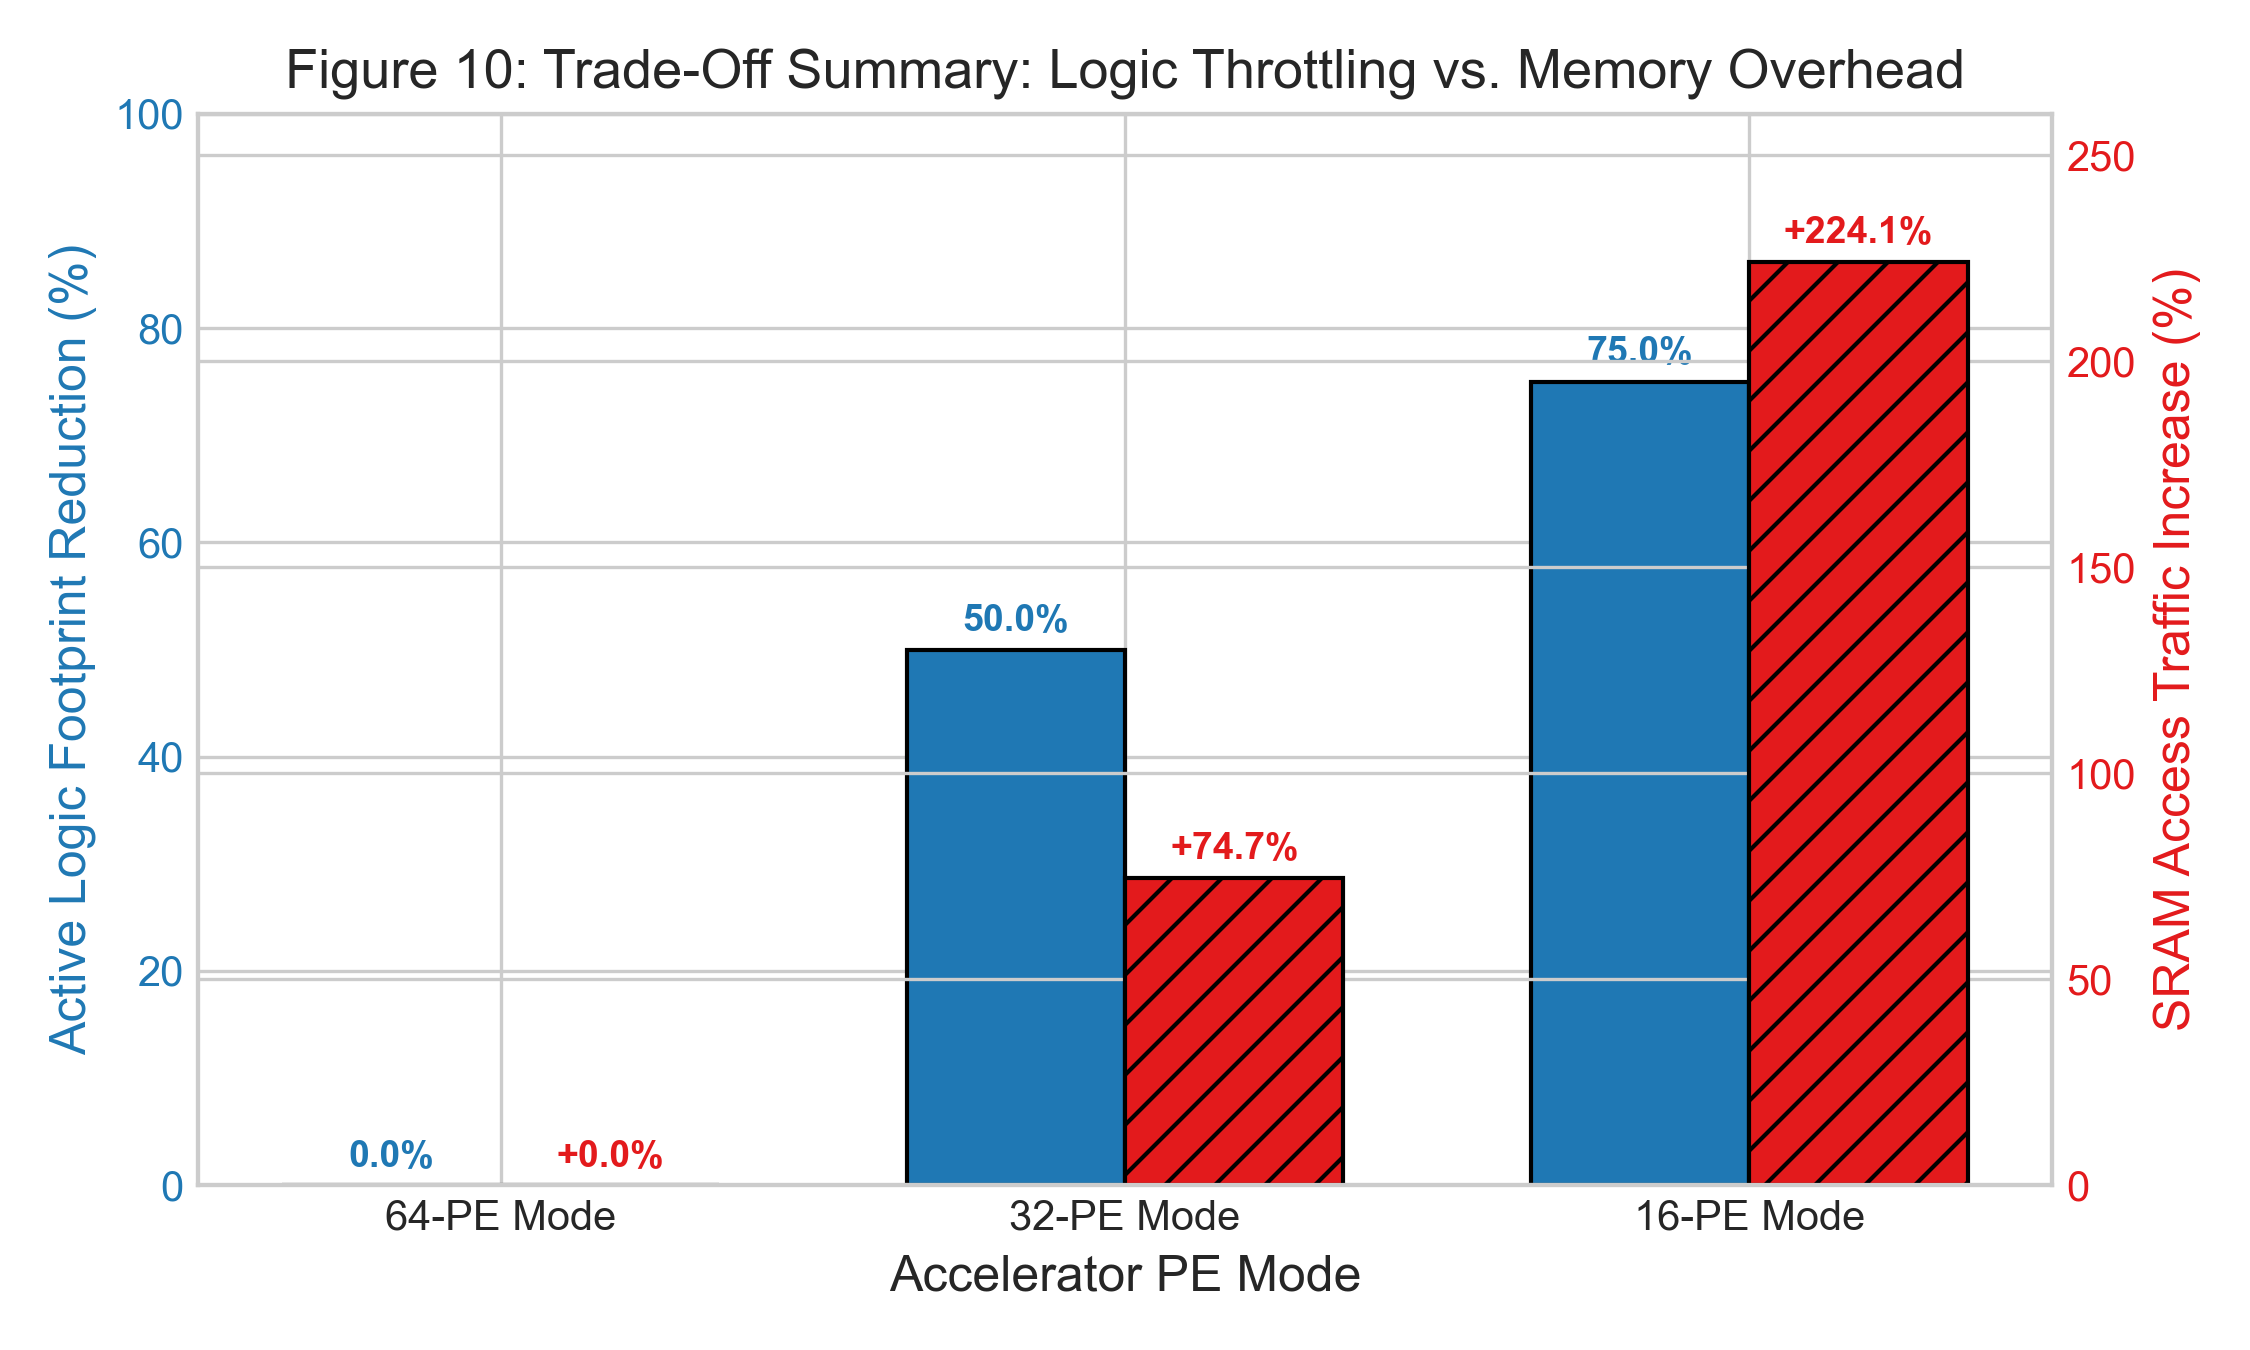
\includegraphics[width=0.96\linewidth]{poster_results_chart.png}
\vspace{0.2em}
\figcaption{Architectural trade-off: Latency, Sparsity savings, and SRAM read inflation.}
\raggedright
\vspace{0.2em}
\textbf{Analysis:} Synchronous zero-gating eliminates weight reads in exact proportion to activation sparsity (ResNet-18 deep layer: 1,390 reads vs. 9,216 baseline). However, down-scaling to 16 PEs quadruples runtime ($4.00\times$) and inflates total SRAM access traffic by \textbf{+224.07\%}, proving that PE throttling must balance peak power against memory bandwidth limits.
\end{posterblock}
\end{minipage}%
\hfill
\begin{minipage}[t]{0.488\textwidth}\vspace{0pt}
\begin{posterblock}[equal height group=rowB]{6}{Positioning vs Existing Work}
\centering
{\bodysize
\renewcommand{\arraystretch}{1.2}
\begin{tabular}{@{}lcccc@{}}
  \toprule
  \textbf{Capability / Metric} & \textbf{Eyeriss} & \textbf{SCNN} & \textbf{NullHop} & \textbf{Ours (Neural\_Acc)} \\
  \midrule
  Sparsity Exploited          & Act & Wt \& Act & Act & \textbf{Activations} \\
  Timing Determinism (0 Jitter)& \yes & \no & \no & \textbf{\yes\ (0.00\% Jitter)} \\
  Configurable PE Scaling     & \no  & \no & \no & \textbf{\yes\ (16/32/64 PE)} \\
  Active Logic Saved          & 0\%  & 0\% & 0\% & \textbf{50.0\% / 75.0\%} \\
  Memory Read Tax Measured    & \no  & \no & \no & \textbf{\yes\ (+100\% / +300\%)} \\
  Hardware Policy Engine      & \no  & \no & \no & \textbf{\yes\ (Single-Cycle)} \\
  Provable Safety Interlock   & \no  & \no & \no & \textbf{\yes\ ($P_{\max}<16$)} \\
  Bit-Exact Equivalence (MAE) & --   & --  & --  & \textbf{0.000000 (100\%)} \\
  \bottomrule
\end{tabular}\par}
\vspace{0.2em}
{\smallsize\color{iitgray}\yes\ supported \quad \partly\ partial \quad \no\ not supported\par}
\raggedright
\vspace{0.3em}
\textbf{Our position:} Only Neural\_Acc resolves the fundamental tension between activation sparsity and real-time determinism while introducing single-cycle hardware policy arbitration and quantifying the multi-pass memory read tax.
\end{posterblock}
\end{minipage}

% ======================== 7 + CONCLUSION ========================
\begin{minipage}[t]{0.488\textwidth}\vspace{0pt}
\begin{posterblock}[equal height group=rowC]{7}{Key Learnings}
\begin{itemize}
  \item \textbf{Technical:} Mastered synthesizable SystemVerilog RTL, Q4.12 fixed-point representation, 40-bit accumulator headroom analysis, and multi-bank SRAM arbitration.
  \item \textbf{Research:} Learned to rigorously challenge published assumptions: throttling active arithmetic units does not imply proportional energy savings once on-chip memory access overheads are accounted for.
  \item \textbf{Engineering / Process:} Built a production-grade regression framework with \textbf{12,202 functional assertions} across 20 testbenches, catching corner-case bugs early before synthesis.
\end{itemize}
\end{posterblock}
\end{minipage}%
\hfill
\begin{minipage}[t]{0.488\textwidth}\vspace{0pt}
\begin{posterblock}[equal height group=rowC]{}{Conclusion and Future Work}
\begin{itemize}
  \item Neural\_Acc successfully decouples power reduction from timing jitter, achieving up to 84.92\% switching savings with zero cycle variation.
  \item Proved that dynamic resource allocation must evaluate holistic memory traffic rather than isolated datapath switching.
  \item \textbf{Next Steps:} TSMC 28nm standard-cell ASIC layout; automated DMA scatter-gather engine for end-to-end ImageNet classification; dual weight-activation sparsity via Compressed Sparse Column (CSC) indexing.
\end{itemize}
{\smallsize
\subhead{Key References:}
[1] Y.-H. Chen et al., \emph{IEEE JSSC}, 2017. \quad
[2] A. Parashar et al., \emph{ACM/IEEE ISCA}, 2017. \quad
[3] T. Chen et al., \emph{ACM ASPLOS}, 2014.\par
\subhead{Acknowledgements:} Department of Computer Science and Engineering, IIT Tirupati.\par}
\end{posterblock}
\end{minipage}

% ======================== FOOTER ========================
\vfill
\begin{tcolorbox}[enhanced, colback=iitmaroon, colframe=iitmaroon, arc=0pt,
  boxrule=0pt, left=16pt, right=16pt, top=7pt, bottom=7pt,
  fontupper=\affilsize\color{white}]
\textbf{M.Tech Project Poster Presentation 2026} \hfill
Department of Computer Science and Engineering, Indian Institute of Technology Tirupati
\end{tcolorbox}

\end{document}
